\subsection{Openstack: a toolkit for building cloud}

\begin{itemize}

	\item Open source project.

	\item Composed of several components (nova, swift, Quantum, Glance, ...) written in Python.

	\item No dynamic scheduling.

	\item Use an AMQP (Advanced Message Queuing Protocol) for inter-components communication.

\end{itemize}



\subsection{DVMS: a dynamic scheduler for virtual machines}

\begin{itemize}

	\item Dynamic scheduler for virtual machines.

	\item Leverage a locality aware p2p overlay.

	\item Successfuly tested in simulator (simgrid) and computing grid (grid'5000).

\end{itemize}


\subsection{Integration of DVMS in Openstack}

\begin{itemize}

\item We propose to replace "nova-scheduler" (static scheduler) by DVMS.

\item Use of an "Adapter" object that will wrap DVMS and integrate well with Openstack, as described in figure \ref{fig:integration}
	\begin{itemize}
		\item It will consume messages that are destinated to "nova-scheduler"

		\item Each message will be converted to a "Dvms" message.
		
		\item Each message produced by Dvms will be converted to an Openstack message and added to the Queue.

	\end{itemize}

\begin{figure*}
	\centering
	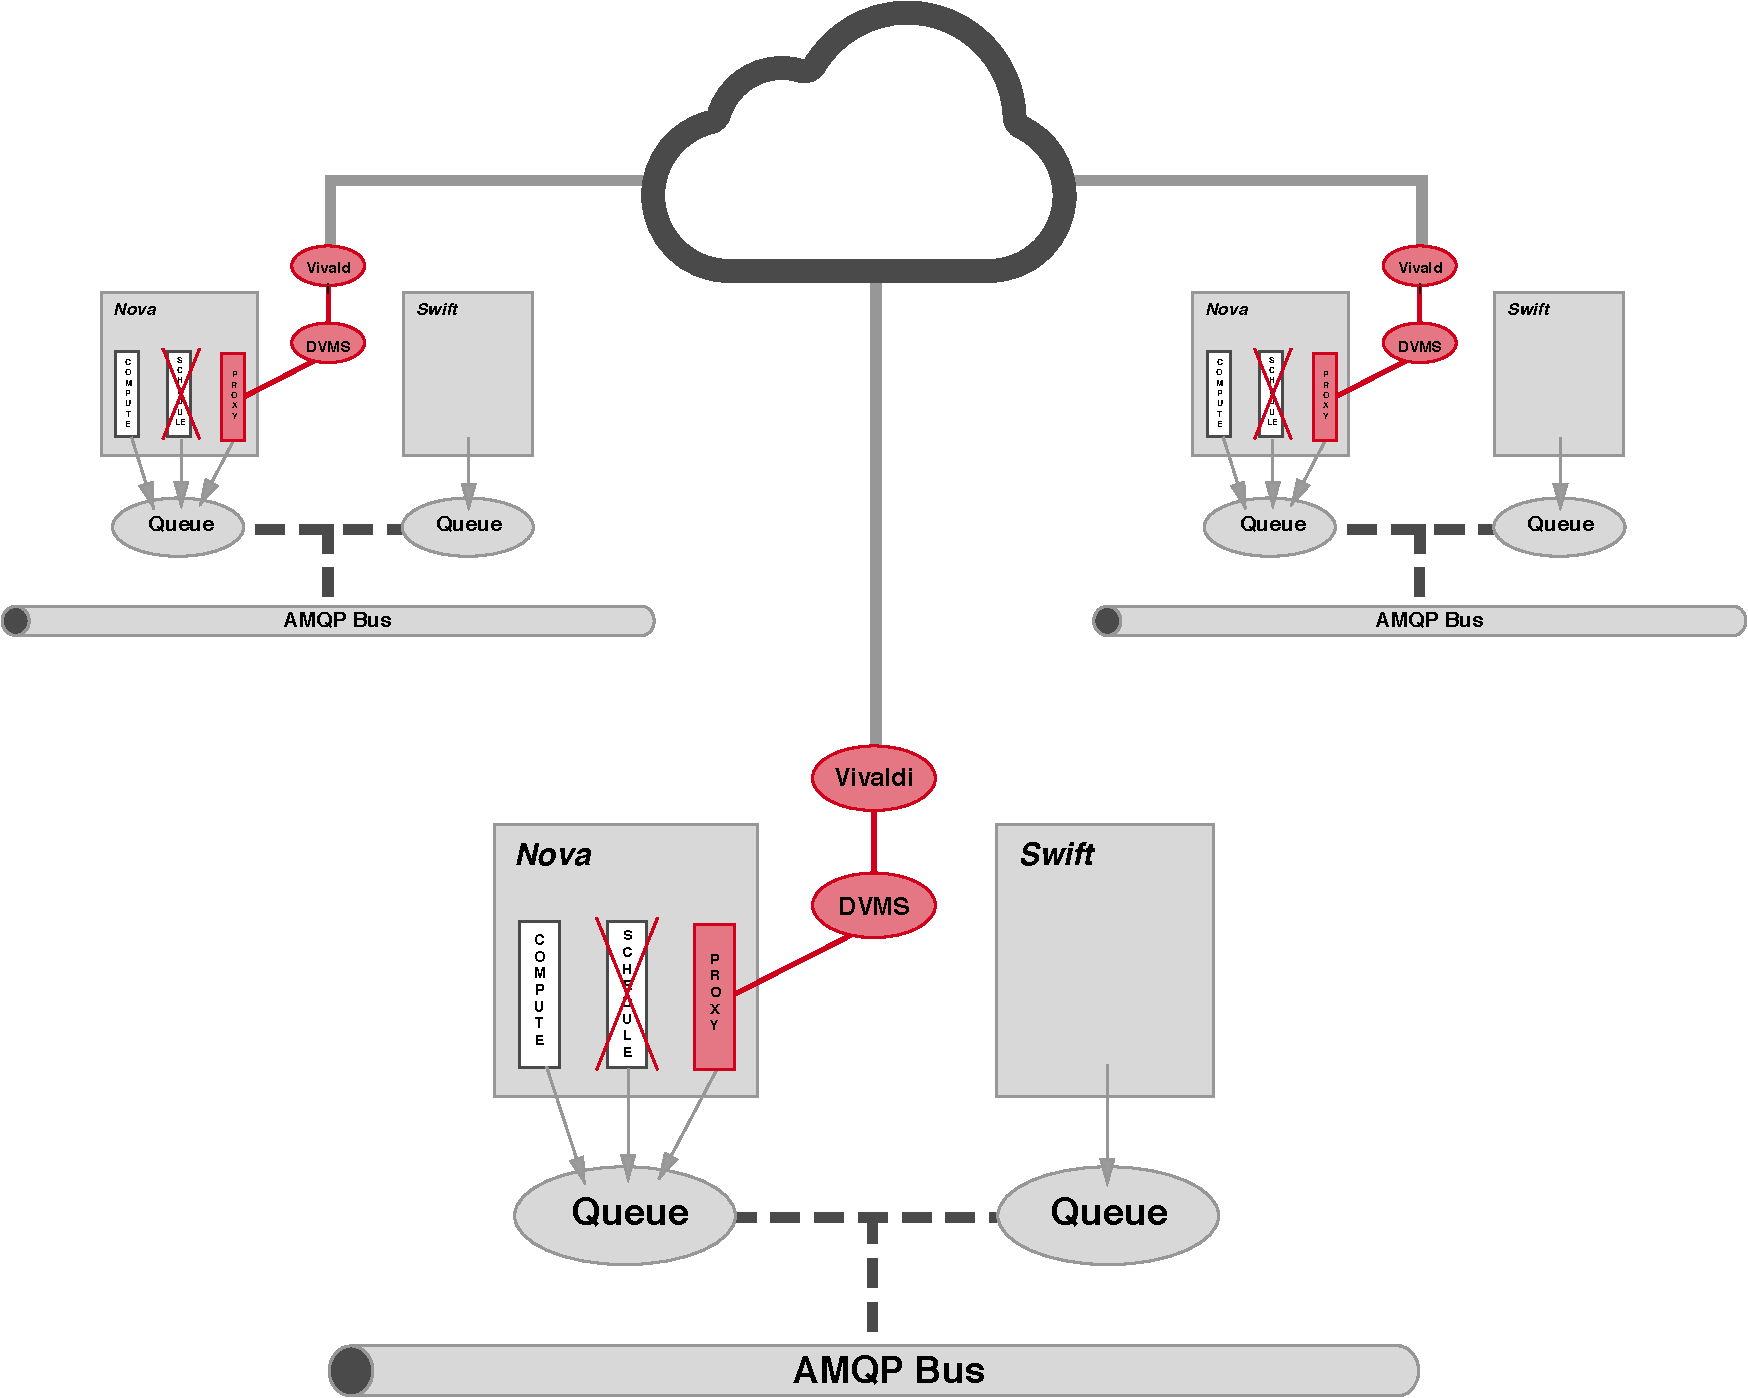
\includegraphics[width=0.75\linewidth]{Figures/openstack_dvms.pdf}
	\caption{Integration of DVMS in Openstack.}%
	\label{fig:integration}%
	%\vspace*{-.8cm}
\end{figure*}

\end{itemize}